\documentclass[12pt]{exam}

\newcommand{\course}{MTH 234 Summer 2021}
\newcommand{\qdate}{12.6 Cylinders and Quadric Surfaces} %PUT DATE HERE
\newcommand{\quiz}{Group Work} 

    \usepackage[top=1in, bottom=1in, left=.45in, right=.45in]{geometry}
    \usepackage{amsmath,amsthm,amssymb,amstext}
    \usepackage{enumerate,enumitem}
    \usepackage{tikz,float,graphicx}
    \usepackage{microtype}
    \usepackage{bm,tikz}
        \usetikzlibrary{calc,positioning}
    \usepackage{multicol}
    \usepackage{nicematrix}
    \usepackage{cleveref}
    \usepackage[framemethod=tikz]{mdframed}
    \usepackage{graphicx}
    \usepackage[export]{adjustbox}
    
    %\newcommand{\course}{MTH 234 Summer 2021}
    %\newcommand{\qdate}{Equations of lines and planes} %PUT DATE HERE
    %\newcommand{\quiz}{Group Work} 
    
    \newcommand{\R}{\mathbb{R}}
    
    \newcommand{\ba}{\bm{a}}
    \newcommand{\bb}{\bm{b}}
    \newcommand{\bc}{\bm{c}}
    \newcommand{\bi}{\bm{i}}
    \newcommand{\bj}{\bm{j}}
    \newcommand{\bk}{\bm{k}}
    \newcommand{\br}{\bm{r}}
    \newcommand{\bv}{\bm{v}}
    \newcommand{\bu}{\bm{u}}
    \newcommand{\gen}[1]{\left\langle #1 \right\rangle}
    \newcommand{\pd}[2]{\dfrac{\partial #1}{\partial #2}}

\newtheorem*{theorem}{Theorem}
\surroundwithmdframed[]{theorem}

\theoremstyle{definition}
    \newtheorem*{definition}{Definition}
    \surroundwithmdframed[]{definition}
    \newtheorem*{info}{Useful Information}
    \surroundwithmdframed[]{info}
\theoremstyle{remark}
    \newtheorem*{remark}{Remark}
    \surroundwithmdframed[]{remark}
    

%%%%%%%%%%%%%%%%%%%%%%%
% HEADER AND FOOTER
%%%%%%%%%%%%%%%%%%%%%%%
\pagestyle{headandfoot}
\firstpageheadrule
\runningheadrule
\firstpageheader{\course}{\quiz}{\qdate}
\runningheader{\course}{\quiz}{\qdate}
\runningfooter{}{}{}


\usepackage{color}
\shadedsolutions
\definecolor{SolutionColor}{rgb}{0.8,0.9,1}

\usepackage{pgfplots}
    \pgfplotsset{every axis/.append style={
                    axis x line=middle,    % put the x axis in the middle
                    axis y line=middle,    % put the y axis in the middle
                    axis z line=middle,
                    axis line style={<->}, % arrows on the axis
                    xlabel={$x$},          % default put x on x-axis
                    ylabel={$y$},          % default put y on y-axis
                    zlabel={$z$},
                    grid=both,
                    %xtick={-4,...,-1,1,...,3},
                    %ytick={-1,1,}
    }}
    \pgfplotsset{compat=1.17}


%\printanswers
\noprintanswers

\begin{document}

\section*{12-6: Cylinders and Quadric Surfaces}

\begin{center}
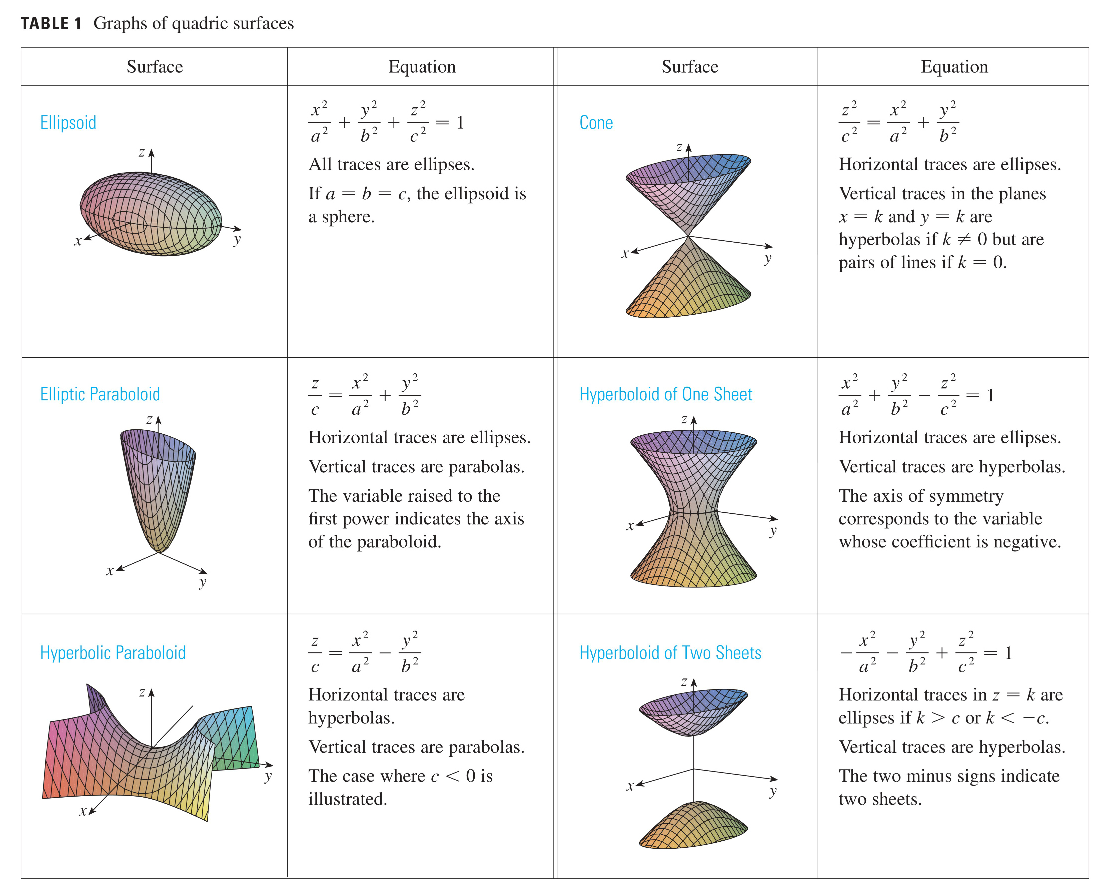
\includegraphics[width=\textwidth]{quadratic_surfaces.pdf}
From Stewart's Calculus 7E
\end{center}

\begin{questions}

\question Classify each curve as a: Cylinder, Ellipsoid, Elliptical Paraboloid, Elliptical Cone, Hyperboloid of one sheet, Hyperboloid of two sheets, or a Hyperbolic paraboloid. 

Draw a sketch demonstrating how each surface is oriented in 3-space. 
    \begin{parts}
    
    \part \(x=y^2+4z^2\)
        \ifprintanswers
            \begin{solution}
                The surface is an elliptic             
            \end{solution}
        \else
            \vfill
        \fi

\newpage 

    \part \(x^2=y^2+4z^2\)
        \ifprintanswers
            \begin{solution}
    
            \end{solution}
        \else
            \vfill
        \fi

    \part \(9x^2-y^2+z^2 = 0\)
        \ifprintanswers
            \begin{solution}
    
            \end{solution}
        \else
            \vfill
        \fi


    \part \(-x^2+y^2-z^2=1\)
        \ifprintanswers
            \begin{solution}
    
            \end{solution}
        \else
            \vfill
        \fi
    \end{parts}
    \newpage

        \begin{center}
            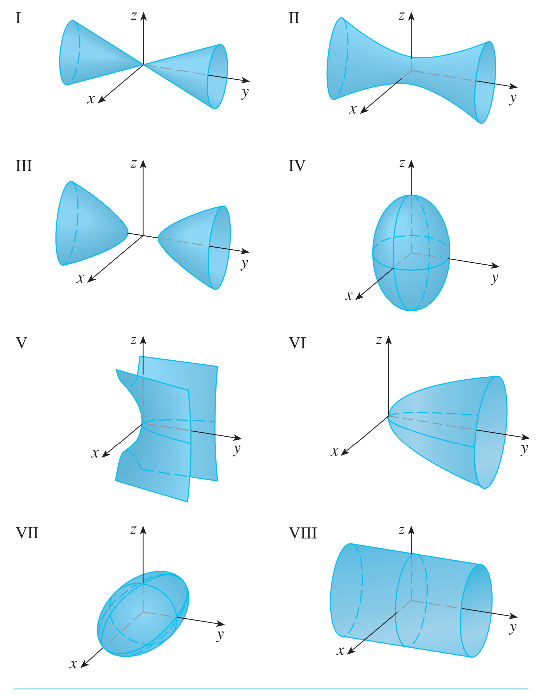
\includegraphics[width=.5\textwidth]{exercises.pdf}

            \emph{From Stewart's Calculus 7e}
        \end{center}

        \question Idenfity the shapes above with the equation that represents them.
        \begin{multicols}{2}
        \begin{parts}
        \part \(x^2+4y^2+9z^2=1\)
        \ifprintanswers
            \begin{solution}
    
            \end{solution}
        \else
            \vspace{1cm}
        \fi

        \part \(9x^2+4y^2+z^2=1\)
        \ifprintanswers
            \begin{solution}
    
            \end{solution}
        \else
            \vspace{1cm}
        \fi

        \part \(x^2-y^2+z^2=1\)
        \ifprintanswers
            \begin{solution}
    
            \end{solution}
        \else
            \vspace{1cm}
        \fi

        \part \(-x^2+y^2-z^2=1\)
        \ifprintanswers
            \begin{solution}
    
            \end{solution}
        \else
            \vspace{1cm}
        \fi

        \part \(y=2x^2+z^2\)
        \ifprintanswers
            \begin{solution}
    
            \end{solution}
        \else
            \vspace{1cm}
        \fi

        \part \(y^2=x^2+2z^2\)
        \ifprintanswers
            \begin{solution}
    
            \end{solution}
        \else
            \vspace{1cm}
        \fi

        \part \(x^2+2z^2=1\)
        \ifprintanswers
            \begin{solution}
    
            \end{solution}
        \else
            \vspace{1cm}
        \fi

        \part \(y=x^2-z^2\)
        \ifprintanswers
            \begin{solution}
    
            \end{solution}
        \else
            \vspace{1cm}
        \fi

        \end{parts}
        \end{multicols}
\end{questions}

\end{document}